\documentclass[12pt]{article} % 12pt 为字号大小 UTF8
\usepackage{amssymb,amsfonts,amsmath,amsthm}
%\usepackage{fontspec,xltxtra,xunicode}
%\usepackage{times}

%----------
% 定义中文环境
%----------

\usepackage{makecell}
\newcommand\toprule{\Xhline{.08em}}
\newcommand\midrule{\Xhline{.05em}}
\newcommand\bottomrule{\Xhline{.08em}}

\usepackage{xeCJK}

% \setCJKmainfont[BoldFont={SimHei},ItalicFont={KaiTi}]{SimSun}
% \setCJKsansfont{SimHei}
% \setCJKfamilyfont{zhsong}{SimSun}
% \setCJKfamilyfont{zhhei}{SimHei}

% \newcommand*{\songti}{\CJKfamily{zhsong}} % 宋体
% \newcommand*{\heiti}{\CJKfamily{zhhei}}   % 黑体


%----------
% 版面设置
%----------
%首段缩进
\usepackage{indentfirst}

\usepackage[shortlabels]{enumitem}

\setlength{\parindent}{2.1em}

%行距
\renewcommand{\baselinestretch}{1.4} % 1.4倍行距

%页边距
\usepackage[a4paper]{geometry}
\geometry{verbose,
  tmargin=3cm,% 上边距
  bmargin=3cm,% 下边距
  lmargin=2cm,% 左边距
  rmargin=2cm % 右边距
}


%----------
% 其他宏包
%----------
%图形相关
\usepackage[x11names]{xcolor} % must before tikz, x11names defines RoyalBlue3
\usepackage{graphicx}
\usepackage{pstricks,pst-plot,pst-eps}
\usepackage{subfig}
\def\pgfsysdriver{pgfsys-dvipdfmx.def} % put before tikz
\usepackage{tikz}

%原文照排
\usepackage{verbatim}

%网址
\usepackage{url}

%----------
% 习题与解答环境
%----------
% %习题环境
% \theoremstyle{definition} 
% \newtheorem{exs}{习题}

% %解答环境
% \ifx\proof\undefined\
% \newenvironment{proof}[1][\protect\proofname]{\par
% \normalfont\topsep6\p@\@plus6\p@\relax
% \trivlist
% \itemindent\parindent
% \item[\hskip\labelsep
% \scshape
% #1]\ignorespaces
% }{%
% \endtrivlist\@endpefalse
% }
% \fi

% \renewcommand{\proofname}{\it{证明}}

%----------
% 我的自定义
%----------

\newcommand{\horrule}[1]{\rule[0.5ex]{\linewidth}{#1}} 	% Horizontal rule

\renewcommand{\refname}{参考文献}
\renewcommand{\abstractname}{\large \bf 摘\quad 要}
\renewcommand{\contentsname}{目录}
\renewcommand{\tablename}{表}
\renewcommand{\figurename}{图}

\setlength{\parskip}{0.4ex} % 段落间距
\usepackage{float}
\usepackage{enumitem}
\setenumerate[1]{itemsep=0pt,partopsep=0pt,parsep=\parskip,topsep=5pt}
\setitemize[1]{itemsep=0.4ex,partopsep=0.4ex,parsep=\parskip,topsep=0.4ex}
\setdescription{itemsep=0pt,partopsep=0pt,parsep=\parskip,topsep=5pt}


%==========
% 正文部分
%==========

\begin{document}
\centerline{\LARGE\textbf{软件学院-2021年春季组合数学 结课报告}} 

\renewcommand\arraystretch{1.5}
\begin{table}[H]
\begin{tabular}{|m{3cm}<{\centering}|m{6cm}<{\centering}|m{2cm}<{\centering}|m{4.5cm}<{\centering}|}

\Xhline{1.1pt}
上课时间 &    2021春季上午     & 讲师 & 冯子铉 \\ 
\Xhline{1.1pt}
学生姓名 & \textbf{张津赫} & 学号 & \textbf{55190815} \\ 
\Xhline{1.1pt}
结课题目&\multicolumn{3}{|l|}{题目}
\\

\Xhline{1.1pt}
\end{tabular}
\end{table}

\vspace{200mm}




\tableofcontents
\thispagestyle{empty}

\newpage
\setcounter{page}{1}

\section{组合数学概述}
\subsection{定义}

组合数学是数学中的一个主要领域,涉及有限或离散系统中的选择,排列和运算问题。它与数学的许多其他领域紧密相关,并且具有从逻辑学到统计物理学,从进化生物学到计算机科学等诸多应用。
\subsection{历史}

\begin{itemize}

\item 中世纪,印度数学家 Mahāvīra (c. 850) 给出了排列与组合的公式,哲学家Rabbi Abraham ibn Ezra (c. 1140) 建立了二项式系数的对称性。
\item 文艺复兴时期,随着数学和自然科学的发展,组合数学的到了新生 Pascal, Newton, Jacob Bernoulli 和 Euler 做出了基础性的贡献,J.J. Sylvester 和 Percy MacMahon建立了计数组合学和代数组合学,便随着四色问题,图论得到了极大的发展。
\item 二十世纪下半叶,组合数学得到了飞速发展,与其他领域的联系更加紧密。
\end{itemize}
\subsection{方法与子领域}
\begin{itemize}

    \item 枚举组合学
    \item 解析组合学
    \item 分区理论
    \item 图论
    \item 设计理论
    \item 概率组合学
    \item 拓扑组合学
    \item 代数组合学
    \item 算术组合学
\end{itemize}






\section{波利亚计数定理}
波利亚计数定理Pólya enumeration theorem用来研究不同着色方案的计数问题,它是组合数学中的一个重要的计数公式,是伯恩赛德引理的一般化,由George Pólya在1937年的论文\cite{GP}中提出并被广泛应用,该结果首先由John Howard Redfield在1927年发表,但当时很少有人能理解,十年后由Pólya独立重新发现。对于含$n$个对象的置换群$G$,用$t$种颜色着色的不同方案数为:

\begin{equation}
\label{eqn:eqn1}
l=\frac{1}{|G|} \sum_{g \in G} t^{c\left(a_{g}\right)}
\end{equation}

其中 $G=a_{1}, a_{2}, \ldots, a_{g}, c\left(a_{k}\right)$ 为置换$a_{k}$的循环指标(Cycle index)数目。

\subsection{母函数形式}
设对$n$个对象用$m$种颜色:$b_{1}, b_{2}, \cdots, b_{m}$着色。设
\begin{equation}
\label{eqn:eqn1}
m^{c\left(p_{i}\right)}=\left(b_{1}+b_{2}+\cdots+b_{m}\right)^{c_{1}\left(p_{i}\right)}\left(b_{1}^{2}+b_{2}^{2}+\cdots+b_{m}^{2}\right)^{c_{2}\left(p_{i}\right)} \cdots\left(b_{1}^{n}+b_{2}^{n}+\cdots+b_{m}^{n}\right)^{c_{n}\left(p_{i}\right)}
\end{equation}

其中${\displaystyle c_{j}(p_{i})}$表示置换群中第$i$个置换循环长度为$j$的个数。

设${\displaystyle S_{k}=(b_{1}^{k}+b_{2}^{k}+\cdots +b_{m}^{k}),k=1,2\cdots ,n}$,则波利亚计数定理的母函数形式为:
\begin{equation}
\label{eqn:eqn1}
P(G)=\frac{1}{|G|} \sum_{j=1}^{g} \Pi_{k=1}^{n} S_{k}^{c_{k}\left(p_{j}\right)}
\end{equation}

波利亚计数定理只是给出计数,但没有给出相应的方案,而母函数形式的波利亚计数定理可以给出相应的方案。








\subsection{波利亚计数定理与伯恩赛德引理的比较}














\begin{itemize}
    \item 波利亚计数定理中的群$G$是作用在$n$个对象上的置换群。
    \item
    伯恩赛德引理中的群$G$是对这$n$个对象染色后的方案集合上的置换群。
    \item
    两个群之间存在一定的联系,群$G$的元素,相应的在染色方案上也诱导出一个属于$G$的置换。
\end{itemize}




















\section{四色定理}
四色定理又称为四色地图定理,是一个著名的数学定理,如果在平面上划出一些邻接的有限区域,那么可以用四种颜色来给这些区域染色,使得每两个邻接区域染的颜色都不一样\cite{newyork}\cite{alex};另一个通俗的说法是:每个无外飞地的地图都可以用不多于四种颜色来染色,而且不会有两个邻接的区域颜色相同。被称为邻接的两个区域是指它们有一段公共的边界,而不仅仅是一个公共的交点。

“是否只用四种颜色就能为所有地图染色?”的问题最早是由南非数学家Francis Guthrie在1852年提出的,被称为“四色问题”或“四色猜想”。人们发现,要证明宽松一点的“五色定理”(即“只用五种颜色就能为所有地图染色”)很容易,但四色问题却出人意料地异常困难。曾经有许多人发表四色问题的证明或反例,但都被证实是错误的。

1976年,数学家Kenneth Appel和Wolfgang Haken借助电子计算机首次得到一个完全的证明,四色问题也终于成为四色定理。这是首个主要借助计算机证明的定理。这个证明一开始并不为许多数学家接受,因为不少人认为这个证明无法用人手直接验证。尽管随着计算机的普及,数学界对计算机辅助证明更能接受,但仍有数学家希望能够找到更简洁或不借助计算机的证明。
\subsection{严格叙述}
四色定理的通俗版本是:“任意一个无飞地的地图都可以用四种颜色染色,使得没有两个相邻国家染的颜色相同。”作为一个数学定理,四色定理有着更为严谨的数学叙述。

    \subsubsection{拓扑学阐述}
    
    最初的染色问题是用几何学的概念描述的,严谨的版本则需要用到拓扑学的概念来定义。设有一平面或其一部分,将其划分为互不重叠的区域的集合。一个“地图”为以下划分方式\cite{rudo}:
\begin{itemize}
\item 将平面划分为有限个区域,使得任意两个区域的交集是空集,所有的区域的并集是整个平面;
\item 所有区域中,只有一个区域是无界区域,其余区域都是有界区域。

\end{itemize}
所谓有界区域,是指能够用一个长和宽都有限的矩形覆盖的区域。无界区域则是不能用这样的矩形覆盖的区域\cite{rudo}。每个区域相当于通俗说法中的“国家”,而区域之间的边界(“国家”之间的“国界线”)则定义为连续不自交的曲线,也称为连续简单曲线。连续简单曲线是指一个从$[0, 1]$映射到平面的连续函数c的像集: $C=\{c(t);\quad t\in [0,1]\}$,并且要满足:

任意$0\leqslant t_{1}<t_{2}\leqslant 1$,只要不是$t_{1}=0,t_{2}=1$,就必定有$c(t_{1})\neq c(t_{2})$
这样说明曲线不与自身相交(没有“打结”的地方)。如果$c(0)\neq c(1)$,就称曲线为弧,否则称曲线为圈\cite{rudo}。可以看出,用边界定义地图更为本质:
平面$\mathbb {R} ^{2}$中的一张地图是指有限个简单曲线的集合:
$\mathcal{L}=\left\{C_{1}, C_{2}, \cdots, C_{m}\right\}, m \in \mathbb{N}, m \geqslant 2$,其中其中$\forall 1\leqslant i\leqslant m,\,C_{i}=\{c_{i}(t);\quad t\in [0,1]\}$
$c_i$为$[0, 1]$映射到$\mathbb {R} ^{2}$的连续函数。并且任意$1\leqslant i<j\leqslant m$,曲线$C_i$和$C_{j}$要么没有交点(交集为空集),要么交点是两线的一个公共顶点$E_{i, j}=c_{i}\left(\epsilon_{1}\right)=c_{j}\left(\epsilon_{2}\right), \quad \epsilon_{1}, \epsilon_{2} \in\{0,1\}$\cite{rudo}

$\mathcal{L}$中每一条连续简单曲线称为地图的边。任意边的端点称为顶点。可以说,一张地图实际上是由一个简单有界平面图定义的。定义地图的边和顶点后,设所有属于边或顶点的点为中性点,其集合设为$\mathcal{N}_{\mathcal{L}}=\left\{x ; x \in C_{i}, 1 \leqslant i \leqslant m\right\}$
则 $\mathcal{L}$将其余的点划分为若干个道路连通的开集。用拓扑学的语言来说,每个“国家”是$\mathbb{R}^{2}-\mathcal{N}_{\mathcal{L}}$的一个极大连通子集。或者说,取一个非中性点x,所有能够从x,经过一条不含中性点的弧到达的点构成的集合,就是一个国家。这样定义的国家必然满足之前所说的特性,只有一个无界国家。要注意的是这里定义的国家必然是没有飞地的。

最后可以定义染色。假设将使用到的颜色编号为$1,2,3,\cdots ,n$号颜色,为地图染色是指一个将地图中的国家映射到$\{1,2,3,\cdots ,n\}$上的函数。一个可行的$n-$染色方案是指使得相邻的国家对应的颜色不同的函数。四色定理说明:每个地图都存在可行的$4-$染色方案[2]:43。
\subsubsection{图论阐述}

拓扑学版本的四色问题阐述可以转化为更为抽象的图论版本。这里的转化指的是一种对偶的概念。即将一个地图转化为图论中的一个无向平面图。具体来说,是将地图中的每一个国家用其内部的一个点代表,作为一个顶点。如果两个国家相邻,就在两个顶点之间连一条线。这样得到的图必然是一个平面图(不会有两条边相交),而与每个国家选取的代表点无关。四色定理可以叙述为:必然可以用四种颜色给平面图的顶点染色,使得相连的顶点颜色不同\cite{rudo}。

要注意的是,并非所有的地图都可以转化为图论中的平面图。如果一个国家有飞地的话,就不能用只一个点来代表一个国家。另外,如果一个国家是“国中国”,那么即便可以地图其转化为平面图,也会造成讨论上的不便。但是,“国中国”的着色十分容易解决,因为它只有一个邻国,只需将它染成和邻国不一样的颜色就可以。所以在大部分有关四色问题的讨论中可以忽略“国中国”的情形。同样地,只有两个邻国的情形也可以被忽略。如果规定不能够有四个或者以上的国家有公共边界,那么地图转化成的平面图里面,每个区域都是至多由三条边围成的。这样的地图被称为正规地图。如果任何一个顶点都连出三条边,那么就称其为“三度图”(trivalent map)。可以证明,如果存在四色定理的反例,那么国家数最少的反例必定是三度图。因此在四色问题的证明过程中,常常会假设地图对应的图是三度图\cite{rudo}。
\begin{figure}[H]
\centering
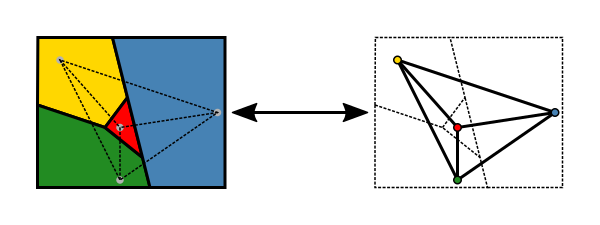
\includegraphics[width=\textwidth]{Four_Colour_Planar_Graph.svg.png}
\caption{一个四个国家的地图转化为一个平面图}
\label{fig:fig1}
\end{figure}


\subsection{肯普的证明思路}

肯普的证明是基于对国家数目进行的归纳法。很容易能证明国家数 4 以内时四色定理成立。肯普假设当国家数目不多于n时四色定理成立,他的目的是证明n+1个国家构成的地图都可以约化为不超过n个国家构成的地图,从而证明四色定理成立\cite{NBK}\cite{PRB}。

肯普首先证明一个有关平面图的结论:任意地图中必定存在一个国家(顶点),其邻国数目小于等于5。证明很简单,在图论版本中,地图被转换成简单平面图。而一个简单平面图中,设$V$为顶点数,$E$为边数,$F$为区域数,则由于每个区域至少由三条边围成,每条边正好隔开两个区域,所以区域数和边数满足:$2E$$\geq$$3F$。假设每个顶点都至少有6条边,那么由于每条边对应两个顶点,所以顶点数和边数满足:$2E$$\geq$$6V$。合起来就有:

\begin{equation}
\label{eqn:eqn1}
V+F \leqslant \frac{1}{3} E+\frac{2}{3} E=E
\end{equation}

但这与图论中著名的欧拉公式:$V$ + $F$ = $E$ + 2矛盾。因此不可能每个顶点都至少有六条边,也就是说,必定有一个国家的邻国数目不超过\cite{alex}。

接下来肯普考察$n+1$个国家中邻国数目最小的国家,称之为A国。A国邻国的数目不超过5个。如果A国的邻国数目不超过3个,那么可以把A国“去掉”(比如和其中一个邻国连成一体),形成一个n个国家的地图,这个地图可以用4种颜色着色,而原来的3个邻国至多用了3种颜色。这时候将A国“放回去”,染上第4种颜色,就等于找到给原地图4-着色的方法\cite{PRB}。

这种能够“去掉”一个国家,减少国家数的局部后来被称为“可约构形”(reducible configuration)。接下来肯普证明A国有4个邻国和5个邻国的情况仍然是可约构形,于是都能够化为不多于n个国家的情况。因此任何n+1个国家的地图仍然可以用四种颜色染色,因而通过归纳法可知,四色定理成立\cite{NBK}。

A国有4个邻国的时候,假如有两个邻国同色,那么可以把它们“当作”同一个国家,和A国连成一体进行约化,而由于此时这4个邻国至多用了3种颜色,所以可以将A国“放回去”,染上第4种颜色。假如4个邻国都不同色,不妨设为红、黄、蓝、绿(如右图2)。肯普的思路是将其转化为两个邻国同色的情形,他采用的方法后来被称为“肯普链”方法(Kempe chain)。具体来说,肯普希望将其中一个邻国的颜色换成“对面”的颜色,比如将绿色(图2中的绿1)换为红色。如果绿色邻国没有红色的邻国,那么换色没有任何问题;如果它有红色邻国(图2中的红1),那么需要将其红色换成绿色,……如此换下去。因此需要换色的是一条绿-红-绿-红……的“链条”,也就是所谓的“肯普链”。如果对面的红色国家不在这个链条里,那么只需要将链中的国家红绿互换,就能转化成两个邻国同色的情况(图3)。如果对面的红色国家也在链条里面(如图4),那么红绿互换就没有意义了。但是这时候可以看到,红绿“肯普链”与A国形成一个圈,所以黄色邻国和蓝色邻国必有一个在圈里(图4中是黄色邻国)。这样圈外的(蓝色)邻国的“肯普链”与圈内的(黄色)邻国必定没有交集,于是将其黄蓝互换,就能转化成两个邻国同色的情况。这说明A国与4个邻国构成可约构形\cite{alex}\cite{NBK}。

对于A国有5个邻国的构形,肯普仍然使用肯普链的换色方式来证明其可约性。他使用了两次换色,将5种颜色降至3种,从而成为可约的构形。这也是后来希伍德找出错误的地方。

\begin{figure}[H]
\centering
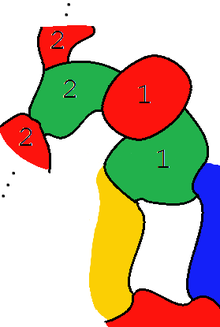
\includegraphics[scale=0.7]{01.png}
\caption{}
\label{fig:GVT}
\end{figure}

\begin{figure}[H]
\centering
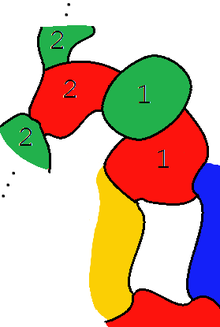
\includegraphics[scale=0.7]{02.png}
\caption{}
\label{fig:GVT}
\end{figure}


\begin{figure}[H]
\centering
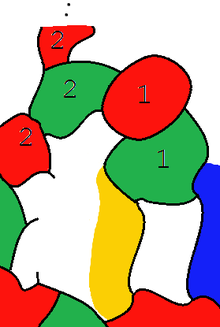
\includegraphics[scale=0.7]{03.png}
\caption{}
\label{fig:GVT}
\end{figure}

\subsection{放电法}

放电法利用地图转换成图染色后成为平面图的特性,将其看作是平面的“电网”,并将每个“节点”按照度数(连出的边数)分类。首先在每个度数为$k$的节点放置6$-$ $k$的电荷。根据平面图和极小五色地图的特性,有下列恒等式:

\begin{equation}
\label{eqn:eqn1}
A_{5}-A_{7}-2 A_{8}-3 A_{9}-\cdots-(s-6) A_{s}=12
\end{equation}

其中$\forall k \in \mathbb{Z}, A_{k}$表示度数为k的节点个数,s为节点最大度数。“放电”的过程(discharging procedure)指的是将这些电荷以特殊的规则进行重新分配,从而找出“电网”结构上的特性,建立不可避免集。具体来说,可以假设某些构形全不存在,然后构造一个放电过程,使得接受电荷的总量不再等于释放电荷的总量,从而导出矛盾(电荷不守恒)。每个良好设计的放电过程都能证明一个不可避免集的存在\cite{JPM}。

\subsection{定理的证明}

1975年,哈肯找到一种很好的放电过程,但难以化为算法程序。于是两人暂时开始回归纸笔计算。这时候他们得到当时还是博士学生的约翰·科赫(英语:John Koch)的支持,后者对他们提供了可约性验证算法工作上的帮助。1976年3月,他们终于得到一个由1936个构形组成的不可避免集,对应的放电过程由487条规则构成\cite{GAY}。同时伊利诺伊大学的主电脑也更换成运算速度更高的IBM 360,为计算节省大量时间。经过电脑1200小时的验证,他们终于在6月得出:1936个构形都是可约构形。这代表着四色定理最终的解决。这时候他们的几个竞争对手如阿莱尔、斯瓦特等的工作也将近尾声。

1976年6月22日,哈肯和阿佩尔首次在美国数学协会(M.A.A.)于多伦多大学召开的美国数学学会(A.M.S.)夏季会议公布他们的结果。不久,伊利诺伊大学数学系的邮戳上加上了“四种颜色就够了”(FOUR COLORS SUFFICE)的一句话,以庆祝四色猜想得到解决\cite{GAY}\cite{POST}。9月,美国数学学会的公告专栏上刊登了两人证明四色定理的消息\cite{APPEL}。

1977年,哈肯和阿佩尔将结果写成名为《任何平面地图都能用四种颜色染色》(Every planar map is four colorable)的论文,分成上下两部分,发表在《伊利诺伊数学杂志》(Illinois Journal of Mathematics)上\cite{APPEL2}\cite{APPEL3}。

\subsection{曲面地图染色}
四色问题探讨的是平面上地图的染色问题。更一般的情况:曲面上地图的染色问题是由希伍德开始研究的。他在1890年的论文中不仅指出肯普的错误,而且运用肯普的方法证明了五色定理。在此之后,希伍德又将注意力转移到更一般的曲面染色问题上。他证明能够对$S_{k}$上面任何的地图进行染色,使得相邻两国不同色所需要的最少颜色数目$\operatorname{Col}\left(S_{k}\right)$有上限:

\begin{equation}
\label{eqn:eqn1}
\operatorname{Col}\left(S_{k}\right) \leqslant\left\lfloor\frac{7+\sqrt{1+48k}}{2}\right\rfloor
\end{equation}


其中的$S_{k}$是指亏格为$k$(有$k$个“洞”)的曲面(或者说二维可微流形),$\left\lfloor \cdot \right\rfloor$ 表示下取整函数。他还证明当亏格为1,也就是曲面为环面的时候,存在至少要用7种颜色才能染色的地图。而环面对应的上限不等式是:
\begin{equation}
\label{eqn:eqn1}
\operatorname{Col}\left(S_{1}\right) \leqslant\left\lfloor\frac{7+\sqrt{1+48}}{2}\right\rfloor=7
\end{equation}

因此希伍德证明了$\operatorname {Col}(S_{1})=7$:最多用7种颜色就能为任何环面上的地图染色\cite{GAY}\cite{GR}。

希伍德猜测,一般的曲面地图染色中,上面的不等式也可以变成等式。他提出猜想:任意的可定向曲面上,最多只用$\left\lfloor\frac{7+\sqrt{1+48}}{2}\right\rfloor$ 种颜色就能为任意的地图染色,其中$k$是曲面的亏格。这个猜想被称为希伍德地图染色问题或者希伍德猜想。当$k = 0$的时候,这个猜想就变成四色猜想。

进一步的推导可以将这个猜想分为12种情况。但仅仅在证明了其中一种和几个较小的$k$的情况后,由于文献上的误导,不少数学家错误地以为问题已经得到解决。1950年后,有关的研究才重新开始。1968年,Gerhard Ringel和John William Theodore Youngs最终证明了这个猜想在$k$ $\geq$ $1$时的情况。而随着1976年,$k = 0$情况(也就是四色定理)的最终证明,希伍德猜想最终获得完整的解决。此后希伍德猜想也开始被称为希伍德地图定理或林格尔-杨格斯定理。





\section{总结与评价}
随着计算机的普及推广,组合数学这门古老的学科焕发出蓬勃的生机。 组合数学是一门研究内容丰富、应用广泛的学科,同时
它也是一门讲究方法,讲究技巧的学科。 组合数学的魅力在于一个组合数学问题的能否得到完善的解决往往取决于能否找到巧妙
的解法,计算机强大的计算能力为寻求组合数学问题的巧妙解法提供了无限的可能,同时组合数学也反过来有效地推动了计算机
科学的发展。

组合数学的理论进展将会深 深地受益于别的数学分
支,猜想代数学的一 些分支,
拓扑学中的一些方法,概率论 方法以及非标准分析方法等都会给组合学的研究提供有效的新工具,同时也会与组合学 结合起来,创造出对其他学 科有用的新方法。
组合数学的发展还会受到 各门应用学科的需要而形成种种带有实际应用色彩的新方 向,例如运筹学、规划论、优化理论与方法、管理数学、 经济数学与生物数学等分支 的发展必将会给组合论提 供新问题,从而也将起着推动组合数学更快发展的作用。















% \section{习题环境}

% \begin{exs}
% 请证明勾股定理。
% \end{exs}
% \begin{proof}
% 这是证明。末尾后会自动添加方块以示结束。
% \end{proof}

% \begin{exs}
% 请计算 $1+2+\ldots +100$。
% \end{exs}
% \begin{proof}[解答]
% 这是解答。末尾后会自动添加方块以示结束。
% \end{proof}

\newpage

\begin{thebibliography}{9}

\addcontentsline{toc}{section}{参考文献}  % 目录中加入参考文献

\bibitem{GP}
G. Pólya. Kombinatorische Anzahlbestimmungen für Gruppen, Graphen und chemische Verbindungen. Acta Mathematica. 1937, 68 (1): 145–254. doi:10.1007/BF02546665








\bibitem{newyork}
  Rudolf Fritsch, Gerda Fritsch. The Four-Color Theorem : History, Topological Foundations, and Idea of proof. Julie Peschke  ISBN 0-387-98497-6
\bibitem{alex}
  Alexander Soifer. The Mathematical Coloring Book: Mathematics of Coloring and the Colorful Life of Its Creators. Springer. 2009 [6 March 2013]. ISBN 978-0-387-74642-5 

\bibitem{rudo}
Rudolf Fritsch, Gerda Fritsch. The Four-Color Theorem : History, Topological Foundations, and Idea of proof. Julie Peschke  New York Berlin Heidelberg: Springer-Verlag. ISBN 0-387-98497-6 

\bibitem{NBK}
Alfred Bray Kempe. On the geographical problem of the four colors. American Journal of Mathematics. 1879年9月3日, 2 (3): 193–200 [2013-03-02].

\bibitem{PRB}
Professors Ralph Bravaco and Shai Simonson. The Four-Color Theorem. Stonehill College. [2013-03-02].

\bibitem{JPM}
Jeremy Preston Magee. Reducible Configurations and So On: The Final Years of the Four Color Theorem. ProQuest. 2008. ISBN 9780549559948 
\bibitem{GAY}
Gary Chartrand, Ping Zhang. Chromatic Graph Theory. CRC Press. 2008年. ISBN 9781584888017 


\bibitem{POST}
Postmarks Used by Department of Mathematics University of Illinois at Urbana-Champaign 

\bibitem{APPEL}
K. Appel, W. Haken. Research Announcement : Every planar map is four colorable. Bull. Amer. Math. Soc. 1976年9月, 82 (5): 711–712
\bibitem{APPEL2}
K. Appel, W. Haken. Every planar map is four colorable. Part I: Discharging. Illinois Journal of Mathematics. 1977, 21 (3): 429–490 

\bibitem{APPEL3}
K. Appel, W. Haken, J. Koch. Every planar map is four colorable. Part II: Reducibility. Illinois Journal of Mathematics. 1977, 21 (3): 491–567

\bibitem{GR}
Gerhard Ringel, J.W.T.Youngs. Solution of the Heawood Map-coloring Problem (PDF). Proceedings of the National Academy of Science of the U.S.A. 1968, 60 (2): 438–445






\end{thebibliography}

\end{document}
